
\begin{questions}
	\question[2] L'évaporation et l'ébullition correspondent au même changement d'état, lequel ?
	
	\fillwithdottedlines{1.5cm}  
	
	\question[2] Sur une courbe qui représente l'évolution de la température en fonction du temps, comment s'appelle la partie horizontale ?
	
	\fillwithdottedlines{1.5cm}  
	
	
	\question[2] Quelle propriété d'un corps ne change pas lorsqu'il change d'état ?
	
	\fillwithdottedlines{1.5cm}  
	
	\question[6] La courbe suivante décrit l'évolution de la température d'un corps lors d'un changement d'état :
	
	\begin{center}
		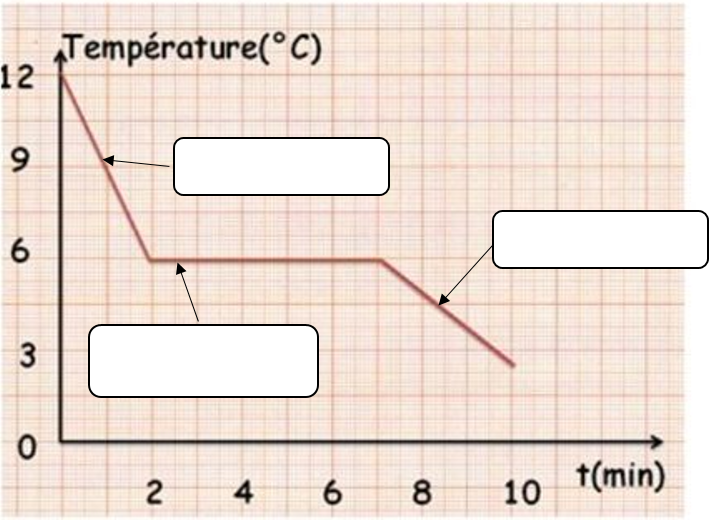
\includegraphics[scale=0.7]{courbe2}
	\end{center}
	
	\begin{parts}
		\part[4] Préciser dans chacun des états indiqués l'état dans lequel se trouve le corps.
		
		\part[2] Quel changement d'état à lieu ici ;
		\fillwithdottedlines{1cm} 
	\end{parts}
	
	
	\question[2] Comment s'appelle le passage de l'état liquide à l'état solide ?
	\fillwithdottedlines{1.5cm}
	
	\question[2] Pendant un changement d'état, la température d'un corps :
	\begin{checkboxes}
		\correctchoice ne change pas
		\choice augmente
		\choice diminue
	\end{checkboxes}
	
	\vspace*{1cm}
	\question[2] Lorsque l'on fournit de l'énergie à de l'eau à 0 °C :
	\begin{checkboxes}
		\correctchoice elle change d'état
		\choice sa température reste constante
		\choice sa température augmente
	\end{checkboxes}
	
	\vspace*{1cm}
	\question[2] Dans des conditions normales de température et de pression, quelle est la température de vaporisation de l'eau ?
	
	\fillwithdottedlines{1.5cm}
	
	
	
\end{questions}

